\begin{figure*}
	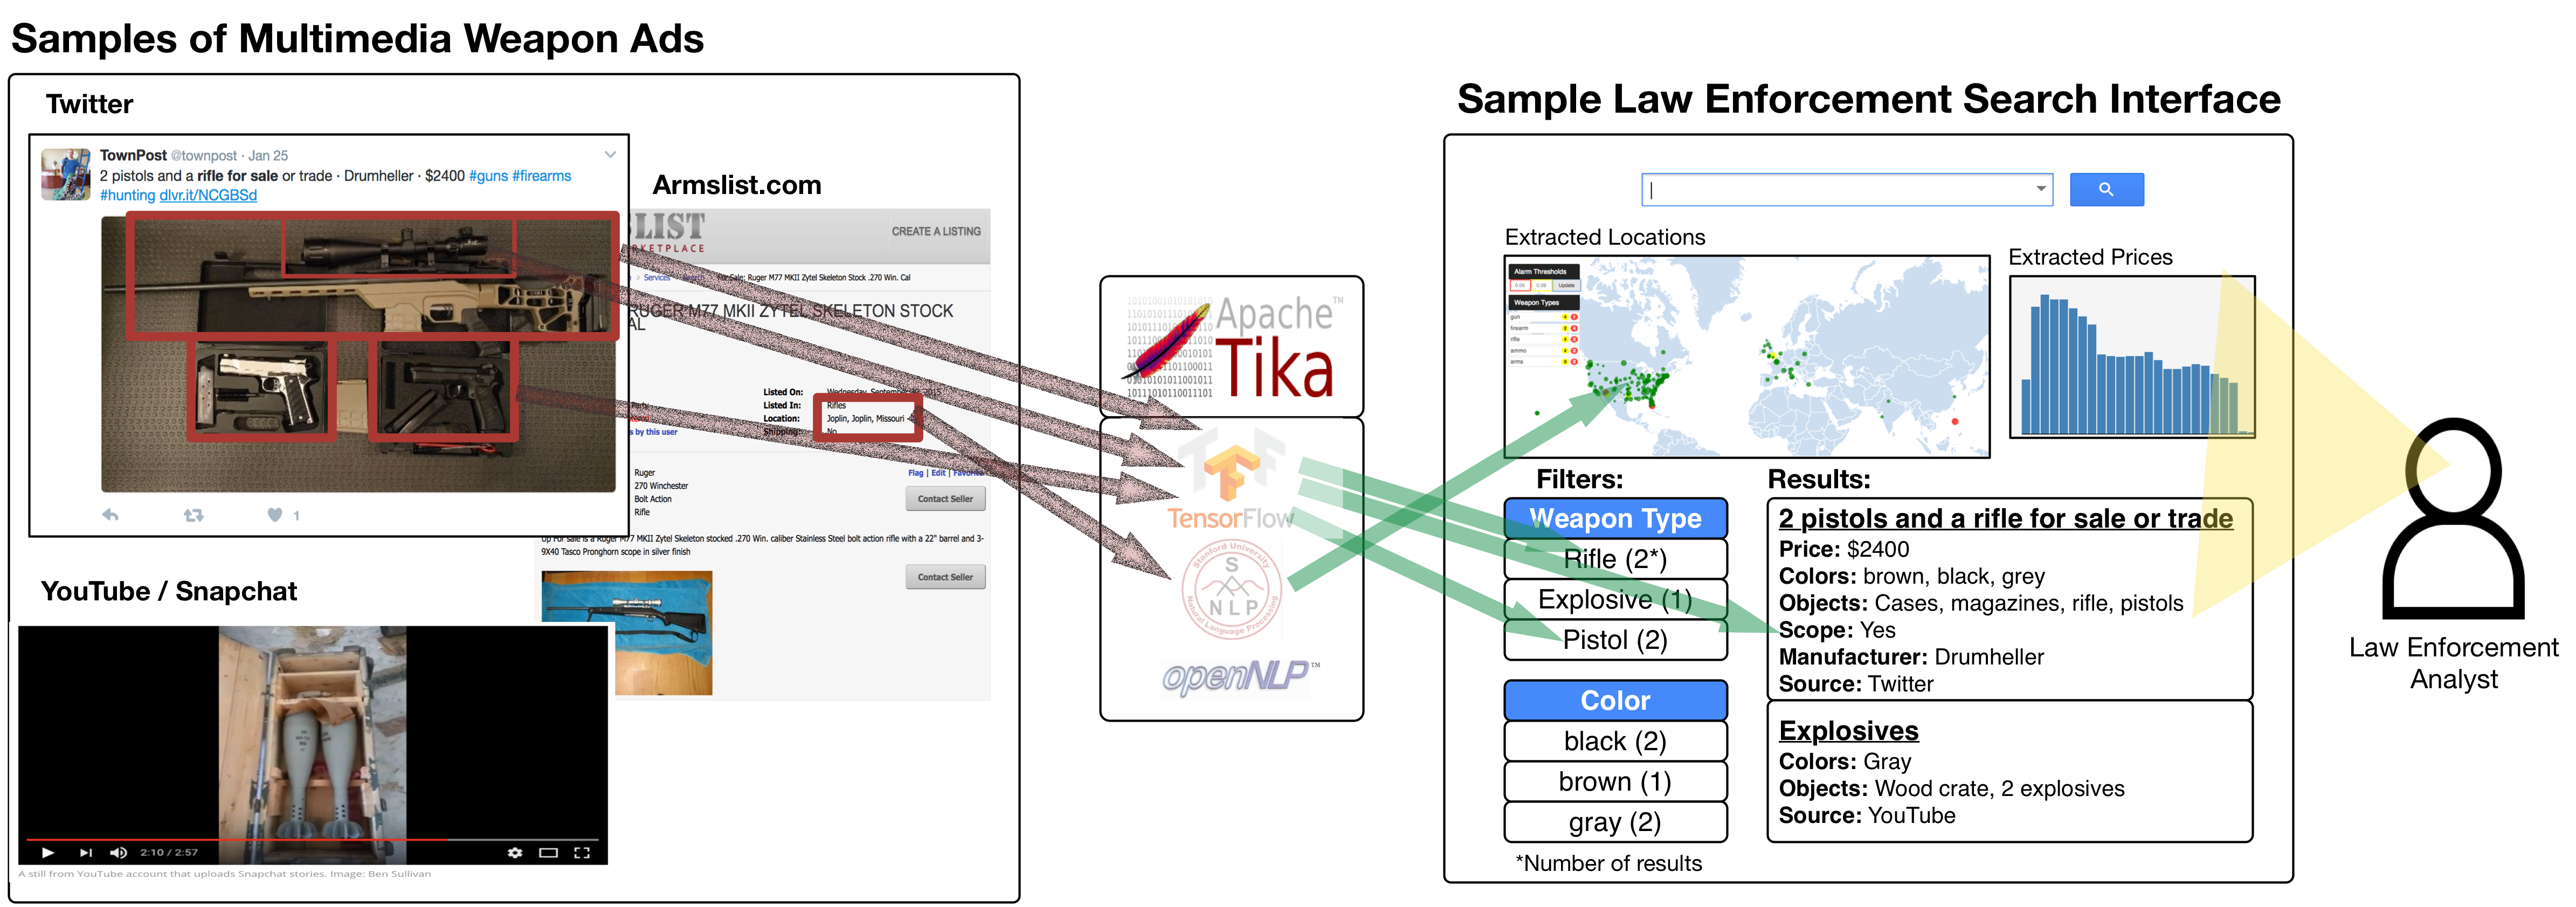
\includegraphics[width=\textwidth,height=6cm]{interface-diagram}
	\caption{This diagram demonstrates how the integration of Tika and Tensorflow facilitates in-depth search across heterogenuous content types. There are several extensions to our object recognition implementation as well, including more refined categories, optical-character recognition, and image similarity metrics.}
	\label{fig:interface-diagram}
\end{figure*}

\section{CONTENT ANALYSIS IN MEMEX PROGRAM} \label{sec:memex}
Law enforcement agencies don't have the manpower to effectively monitor the scale of weapons ads discussed in section \ref{memex-data}. This problem is exascerbated by the fact that important information is often embedded in rich content (images, audio, video) present in these ads. While a majority of web content consists of either plain or rich text \cite{mphillips-EOT2012}, the need for computer vision and pixel-based analysis has increased with the rise of multimedia. Recent work on Apache Tika is continuing to expand capabilities for detecting and analyzing textual information while also expanding its support into deep learning and computer vision frameworks. 

\subsection{Extending Tika into Computer Vision}

On the textual side, Tika has recently added support for information extraction tasks such as named-entity recognition (NER) using popular Natural Language Processing toolkits like Stanford CoreNLP\cite{Finkel:2005:INI:1219840.1219885}, Apache OpenNLP\cite{ApacheOpenNLP}, and MIT Lincoln Lab's MITIE \cite{MITIE-github}. On the computer vision side, and the focus of this paper, Tika now provides support for one of the most popular and well-documented deep learning frameworks, Google's Tensforflow. Specifically, our integration of Tensorflow is focused around object recognition, which allows for the identification of objects of interest in graphical data. 

Historically, the best object recognition systems were inaccruate, but this has changed due to recent advancements in deep neural networks, larger training datasets, and improved computing resources. Tensorflow is a scalable, Python-based system and it natively supports image recognition via its \em {Inception} model \cite{abadi2016tensorflow}. \em{Inception} provides a neural network trained on the ImageNet corpus \cite{krizhevsky2012imagenet}, a dataset of 14,197,122 images and classified using the WordNet taxonomy. The end result is a highly-scable off-the-shelf system that can accuractely identify and classify objects in images into a thousand categories. 

Integration of Tensorflow with Tika presented a significant challenge: Tensorflow does not provide out of the box bindings to Java based frameworks. Apache Tika is primarily written in Java and thus integrating with Tensorflow is not straight forward like any other JVM compatible libraries. In the following sections we explore the pros and cons of various methods of integration.

% Object recognition is a standard problem in computer vision which deals with the recognition of objects of interest in the graphical data. In the context of images it is often called as image recognition. Historically image recognition was a challenging task and its accuracy of the recognized objects were much lower than average Human performance. However, due to the recent advancements in deep neural networks and availability of larger datasets with faster computing resources, we now have systems which have nearer or better performance than average human beings\cite{karpathy-cnn-compare}.

% Today's deep learning frameworks are focused towards performance gain from native code and GPU optimization for fast matrix manipulations. One of the most popular and well-documented deep-learning systems is Google's Tensorflow \cite{abadi2016tensorflow}. Tensorflow is a scalable, Python-based system and it natively supports image recognition via its {\em Inception} model \cite{abadi2016tensorflow}. Inception provides a neural network trained on the ImageNet corpus \cite{krizhevsky2012imagenet}, a dataset of 14,197,122 images and classified using the WordNet taxonomy. As such, Tensor 

\subsection{Tools for Law Enforcement} \label{sec:memex-tools}
The ultimate goal of integrating and characterizing diverse content scattered across the web is to provide law enforcement analysts with tools that will help them quickly identify potentially illegal activity, and multimedia content is key piece of the puzzle. Images and videos often provide salient information not available in text; in many cases, illegal weapons dealers intentionally embed revealing details in rich content mediums because they are harder to identify. This thinking coincides with the rise of weapons trafficking on social media platforms such as Snapchat, YouTube, and Instagram, where communication is centered around images and video \cite{socialmedia}. The integration of Tensorflow and Tika provides a single, streamlined platform that unites the extraction of textual and rich content. This combined content can then be exposed through search and visualization interfaces that improve analysts' abilities to drill-down and explore comprehensive, diverse content contained in weapons ads (see Figure \ref{fig:interface-diagram}). 